\documentclass[11pt, a4paper]{article}
\usepackage[utf8]{inputenc}
\usepackage[ngerman]{babel}
\usepackage{graphicx}

\begin{document}

\tableofcontents
\thispagestyle{empty}
\newpage

\section{Einleitung}
Hier eine kurze Einleitung in welchem Rahmen diese Arbeit entstanden ist und schonmal ganz kurz auf SETI eingehen.

\section{SETI Breakthrough Listen}
Die kaggle Challenge \emph{SETI Breakthrough Listen - E.T. Signal Search} war ein öffentlicher Machine Learning Wettbewerb des \emph{Berkeley SETI Research Centers} im Zeitraum vom 10. Mai 2021 bis 18. August 2021. Die zugrunde liegenden Daten sind noch verfügbar, sodass Interessierte sich nach wie vor mit diesem Problem beschäftigen können. Im folgenden werden wir die Challenge stets abgekürzt als \emph{SETI} bezeichnen. 

Die Herausforderung bei \emph{SETI} besteht darin, Spektrogramme, also eine bildliche Darstellung eines Frequenzbereichs in einem bestimmten Zeitraum, die basierend auf Rohdaten des \emph{Green Bank Telescopes} generiert worden sind, auf das Vorkommen von künstlich hinzugefügten extraterrestrischen Signalen zu untersuchen. Hierbei ist es wichtig, diese Signale von irdisches Signalen, wie etwa einem Radiosignal, zu unterscheiden. Um diese Unterscheidung vornehmen zu können, sind jeweils sechs Spektrogramme zusammengefasst, wobei die Spektrogramme eins, drei und fünf jeweils Aufnahmen des zu untersuchenden Ziels \glqq A\grqq{} sind und die übrigen jeweils auf Aufnahmen eines anderen Himmelskörpers \glqq B\grqq{}, \glqq C\grqq{} und \glqq D\grqq{}. Eine solche Gruppe von Spektrogrammen (ABACAD) wird bei \emph{SETI} als \emph{Kadenz-Ausschnitt}, im folgenden nur noch \glqq Kadenz\grqq{}, bezeichnet.

Abbildung \ref{fig:kadenz_pos_1} zeigt ein Beispiel für eine Kadenz mit einem extraterrestrischen Signal. Auf den drei Spektrogrammen, die auf das Ziel gerichtet sind (in der Abbildung durch \glqq ON\grqq{} gekennzeichnet) ist jeweils ein Signal zu erkennen, welches nicht auf den anderen Spektrogrammen zu sehen ist. Offensichtlich muss ein Signal nicht auf jedem der drei \emph{on target} Spektrogrammen zu sehen sein, da ein Signal nicht zwingend über den gesamten zeitlichen Betrachtungsraum aktiv sein muss.

\begin{figure}[t]
\centering
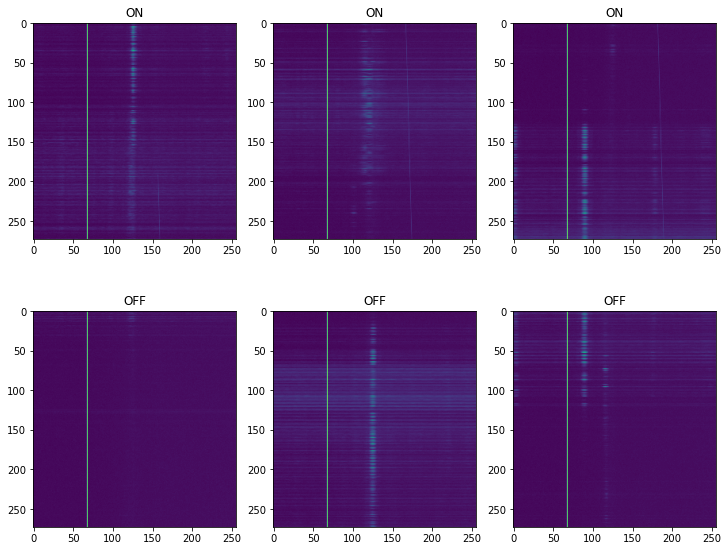
\includegraphics[width=0.9\textwidth]{"img/kadenz_pos_1.png"}
\caption{Beispiel für eine Kadenz mit Nadel}
\label{fig:kadenz_pos_1}
\end{figure}

Die Trainingsdaten für \emph{SETI} enthalten 60.000 Kadenzen (\emph{Heuhaufen}) von denen 6.000 \emph{Nadeln} sind, also Kadenzen, die ein künstlich eingefügtes extraterrestrisches Signal enthalten. Einige dieser Signale sind bei entsprechender Visualisierung sofort mit bloßem Auge zu erkennen, andere sind in, durch irdische Signale verursachten, Rauschen versteckt. Weil die Challenge zum Zeitpunkt der Projektarbeit nicht mehr aktiv ist und die zu den Testdaten der Challenge keine Labels verfügbar sind, müssen wir die Trainingsdaten in Trainings- und Testdaten aufteilen, um ein Modell abschließend auf Testdaten laufen lassen zu können. Hierzu führen wir einen 70/30 Split der Trainingsdaten durch und erhalten danach ein Trainingsset mir 42000 Kadenzen und ein Testset mit 18000 Kadenzen. Dieser Split wird durch einen \emph{Seed} reproduzierbar gemacht, um verschiedene Modelle vergleichen zu können, in dem sie auf dem jeweils selben Split der verfügbaren Daten trainiert und getestet werden.


\section{Implementierung}
Im folgenden beschäftigen wir uns nun mit der Problemlösung für \emph{SETI}. Wir schauen uns erste Ansätze mit reiner Computer Vision an, die uns helfen sollen auch versteckte Signale extrahieren zu können, um sie mit bloßem Auge erkennen zu können. Wir haben uns für diesen Einstieg entschieden, um ein Gefühl für die visuelle Form der gesuchten Signale und für den Datensatz allgemein zu erhalten. Im darauf folgenden Kapitel werden wir uns mit \emph{Convulutional Neural Networks}, kurz \emph{CNNs}, beschäftigen.

\subsection{Erste Ansätze mit Computer Vision}
Wenn man über Bilderkennung spricht denkt man meistens direkt an Machine Learning und Neurale Netzwerke. Allerdings gibt es in der Bilderkennung Problematiken, die sich mithilfe der klassischen Computer Vision deutlich besser lösen lassen. Im Folgenden wird auf die grundlegenden Unterschiede zwischen der klassischen Computervision und Machine Learning eingegangen, einige Grundlagen beschrieben, Lösungen der Computervision angewandt auf die Problematik der Projektarbeit und ob die klassische Computervision für diese Projektarbeit geeignet ist.

\subsubsection{Unterschiede Computervision - Machine Learning}
Computervision ist nicht gleichzusetzen mit Machine Learning. Die klassische Computervision arbeitet mit rein mathematischen Ansätzen und Algorithmen, während das klassische Machine Learning eher darauf bedacht ist mithilfe von Trainingsdaten Modelle zu trainieren und dadurch Parameteranpassungen durchzuführen. Computervision ist sehr vielfältig einsetzbar. Mithilfe von Algorithmen können beispielsweise alle möglichen geometrische Primitive detektiert werden, also beispielsweise Linien und Kreise. Außerdem kann mithilfe von sogenannten Filtern das Bild verarbeitet werden um zum Beispiel bestimmte Elemente im Bild zu eleminieren, das Bild zu schärfen oder zu glätten und noch vieles darüber hinaus. Diese Filter werden außerdem in den nachfolgenden Kapiteln noch sehr interessant für die Convolutional Neural Networks.

\subsubsection{Grundlagen}
Bilder sind im Prinzip nichts weiter als eine große Ansammlung von Zahlen, welche die entsprechenden Farben repräsentieren. In der klassischen Computervision arbeitet man häufig mit sogenannten Grauwertbildern. Diese sind besonders einfach zu handhaben, da diese nur einen Farbkanal besitzen im Gegensatz zu RGB Farbbildern, welche die 3 Farbkanäle Rot, Grün und Blau besitzen.

\subsubsection{Lokale Operatoren: Filter}
Lokale Operatoren sind sogenannte Punktoperationen, also Operationen die auf jedem Pixel des Bildes angewandt werden. Bei Lokalen Operatoren ist die Besonderheit, dass benachbarte Pixel auch mit in die Berechnung der Operation einfließen und somit auch den Farbwert des betrachteten Pixels beeinflussen. Somit können zum Beispiel Grauwertübergänge, also Übergänge von dunkel nach hell, detektiert werden. Um Punktoperationen besser zu verstehen, muss man das Bild als eine drei-dimensionale Funktion betrachten: die x Achse steht für die Breite des Bildes, y ist die Höhe des Bildes und z die Farbe des entsprechenden Pixels an der Stelle (x,y), so erhält man eine Grauwertfunktion g(x,y)=z. An den Stellen wo es einen schnellen Wechsel von dunkel zu hell gibt, hat die Ableitung der Grauwertfunktion einen Extrempunkt. Die Ableitung der Grauwertfunktion lautet:
\newline

g'(x,y)=[$\frac{\partial g(x,y)}{\partial x}$, $\frac{\partial g(x,y)}{\partial y}$]$^T$
\newline
Für diskrete Bilder muss die Ableitung allerdings angenähert werden, da ein Pixel nur einen einzigen Wert beinhaltet:
\newline

$\frac{\partial g(x,y)}{\partial x}$ = $\frac{g(x+\Delta x,y)-g(x-\Delta x,y)}{\Delta x}$
\newline

$\frac{\partial g(x,y)}{\partial y}$ = $\frac{g(x,y+\Delta y)-g(x,y-\Delta y)}{\Delta y}$
\newline
Setzt man nun $\Delta x$ beziehungsweise $\Delta y$ gleich 1 erhält man folgende Approximationen:
\newline

$\frac{\partial g(x,y)}{\partial x}$ = $\frac{g(x+1,y)-g(x-1,y)}{1}$
\newline

$\frac{\partial g(x,y)}{\partial y}$ = $\frac{g(x,y+1)-g(x,y-1)}{1}$
\newline
Für jedes Pixel (x,y) auf welches diese Approximation angewandt wird, wird also folgendes berechnet:
\newline

$1\cdot g(x+1,y)+0\cdot g(x,y)-1\cdot g(x-1,y)$
\newline
Wir erhalten also folgendes Operatorfenster:
\begin{figure}[h]
\centering
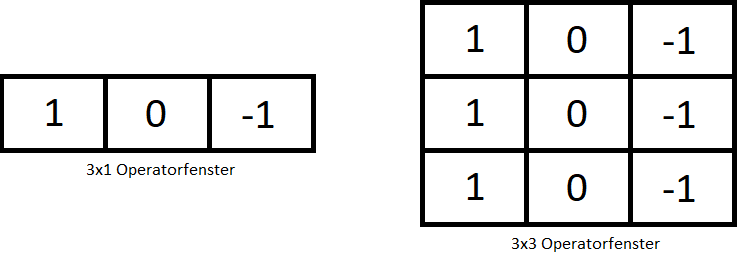
\includegraphics[width=0.9\textwidth]{img/operatorfenster.png}
\end{figure}
\newline
Mit dem Operatorfenster kann auf jedem einzelnen Pixel eine sogenannte gewichtete Addition ausgeführt werden, was genau der oben hergeleiteten Berechnungen entspricht. Dafür legt man das Operatorfenster auf eine entsprechende Stelle des Bildes, multipliziert die einzelnen Komponenten des Fensters mit den darunterliegenden Werten der Pixel und summiert diese Produkte. Anstatt eines 3x1 Operatorfensters können auch 3x3 Operatorfenster genutzt werden, wodurch auch Pixel die über und unter dem zu betrachtenden Pixel mit in die Berechnung einfließen. Das Ergebnis der Anwendung des oben abgebildeten Operatorfensters ist ein neues Bild, welches insbesondere vertikale Grauwertübergänge hervorhebt und horizontale Grauwertübergänge entfernt. Der Grund dafür ist die Approximation der ersten Ableitung in x-Richtung, wodurch die Grauwertfunktion des Bildes abgeleitet wird. Dadurch kann man das resultierende Bild sozusagen als Ableitung des Originalgrauwertbildes betrachten: Stellen die hervorgehoben werden, sind starke Grauwertübergänge und horizontale Linien werden entfernt, da auf einer gleichfarbigen horizontalen Linie keine ausschlaggebenden Veränderungen der Grauwerte vorkommen. Dasselbe gilt umgekehrt für die Approximation in y-Richtung - dafür muss das Operatorfenster einfach nur um 90 Grad gedreht werden. Mit der Approximation in y-Richtung werden allerdings vertikale Linien eleminiert.
\begin{figure}[h]
\centering
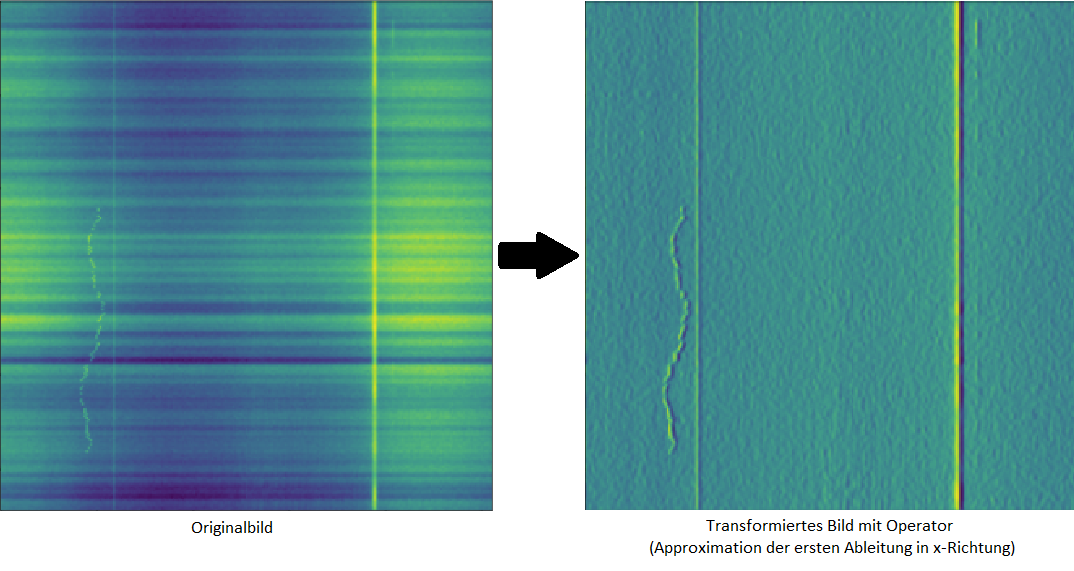
\includegraphics[width=0.9\textwidth]{img/original-vs-cv.png}
\end{figure}
\newline
Die Idee hinter der Verwendung der Filter ist die, dass die Signale alle eine vertikale Richtung aufweisen. Mithilfe der Filter für die Eleminierung der horizontalen Linien kann also Rauschen recht einfach rausgefiltert werden.
TODO: Referenz auf Laubenheimer Folien

\subsubsection{Weitere Experimente}
Das Rauschen in den Bildern ist häufig sehr ausgeprägt, weshalb auch mit Algorithmen zur Rauschminderung experimentiert wurde. Die Idee hinter dem ersten Algorithmus war es ähnliche Pixel auf dieselbe Farbe abzubilden. Anfangs wird die Anzahl der unterschiedlichen Farben gezählt und anschließend die mittlere Differenz der Farbwerte berechnet. Anhand der mittleren Differenz und ein als Parameter festgelegter Wert, der bestimmt wie stark die mittlere Differenz den Algorithmus beeinflusst, kann ein neuer Wert berechnet werden, der bestimmt wie unterschiedlich ähnliche Pixel zueinander sein dürfen, sodass sie auf dieselbe Farbe abgebildet werden. 
\newline
Nachdem nun dieser Algorithmus zur Abbildung ähnlicher Pixel auf dieselbe Farbe angewandt wurde, kann es sein dass die unterschiedlichen Farben teilweise einen geringeren, aber auch einen höheren Abstand zum jeweils nächsten Farbwert haben. Die Lösung dafür ist genau diese Differenz zwischen allen Farbwerten auf die mittlere Differenz zu setzen. Dadurch erreicht man, dass die Farben, die bislang noch sehr nah beieinander lagen, nach Anwendung dieses Algorithmus besser zu unterscheiden sind und Farben, die bislang eher weiter weg voneinander lagen, immer noch gut voneinander unterscheidbar sind. Anfangs wird wieder die Anzahl der unterschiedlichen Farben gezählt und auch die mittlere Differenz zwischen den einzelnen Farben berechnet. Da die Farben nach Anwendung des Algorithmus genau diese mittlere Differenz zueinander haben soll, werden die Farben nacheinander auf jeweils ein Vielfaches der mittleren Farbdifferenz abgebildet.
\newline
Führt man vor diesen beiden Algorithmen den Filter zur Entfernung der horizontalen Linien aus, erhält man beispielsweise folgende Transformation:
\begin{figure}[h]
\centering
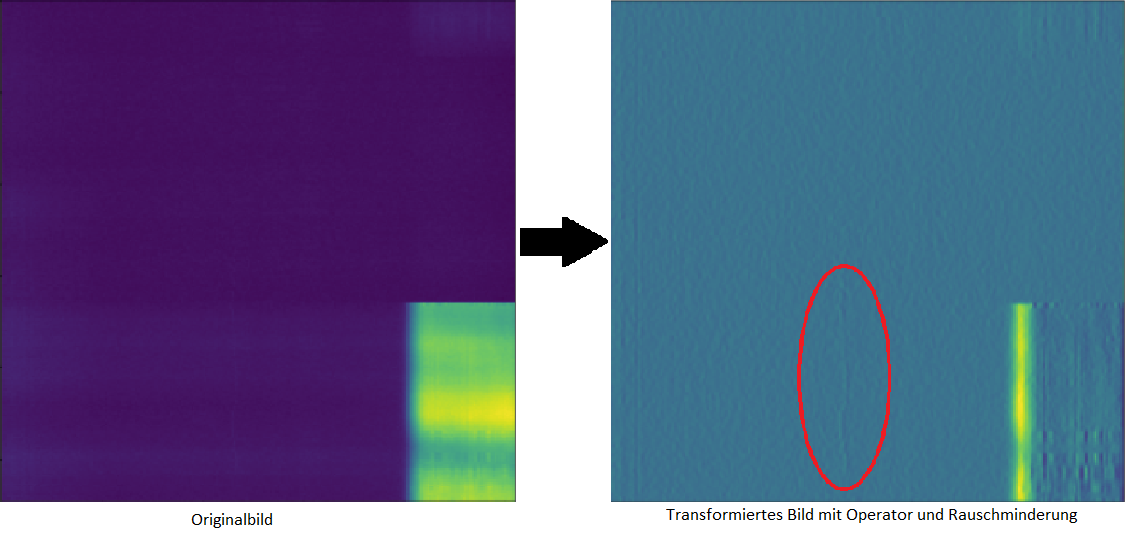
\includegraphics[width=0.9\textwidth]{img/original-vs-rauschminderung.png}
\end{figure}
\newline
Auf dem Originalbild ist mit dem bloßen Auge kein Signal zu finden, betrachtet man allerdings das transformierte Bild ist ein schwaches Signal zu erkennen.

\subsubsection{Zwischenfazit: Computervision alleine bringt keinen Erfolg}
Computervision ist zwar sehr vielfältig einsetzbar, allerdings für die Problematik dieser Projektarbeit nur sehr schwer anwendbar. Das liegt insbesondere daran, dass die Signale teilweise im Hintergrundrauschen sehr gut versteckt sind und teilweise nicht mal mit dem Auge zu erkennen sind. Wie bereits erläutert, kann man zwar mithlife von Filtern und etwas Algorithmik die Signale besser vom Hintergrund hervorheben, allerdings müssten die Signale für eine reine Computervision Lösung detektierbar sein. Dafür hat die Computervision wie bereits am Anfang erwähnt zum Beispiel Möglichkeiten für die Detektion von geometrischen Primitiven. Allerdings sind viele der Signale auch nach Verarbeitung der Algorithmen nur schwer zu erkennen und darüberhinaus ist die Form der Signale unbestimmt, was die Detektion auf Basis von Algorithmen sehr schwer macht. Eine andere Möglichkeit der Detektion ist die Anwendung von Convolutional Neural Networks, worauf in dem nächsten Kapitel näher eingegangen wird.

\section{Deep Learning}
Natürlich wollen wir nicht alle Kadenzen einzeln manuell betrachten und entscheiden, ob sie eine Nadel enthalten oder nicht. Vielmehr wollen wir ein Machine Learning Model trainieren, das uns diese Arbeit abnimmt und Nadeln findet. Hierzu wollen wir ein \emph{Convolutional Neural Network (CNN)} trainieren, das die Kadenzen in genau zwei Klassen einteilt: enthält eine Nadel oder enthält keine Nadel.

\subsection{Convolutional Neural Networks}
Um uns an den Umgang mit \emph{CNNs} heranzutasten, entwerfen wir zunächst ein kleines Netz bestehend aus zwei \emph{Hidden Layern} und einem \emph{Fully Connected Layer}. Die beiden \emph{Hidden Layer} bestehen aus je einem \emph{Convolutional Layer} und einem \emph{Pooling Layer}. Wir teilen die Trainingsdaten noch einmal mit einem Verhältnis von 90 zu 10 in Trainings- und Validierungsdaten. 

Unsere erste Beobachtung ist, dass wir selbst mit einem so kleinen Netz bereits eine sehr hohe \emph{Accuracy} erzielen und sich auch der \emph{Loss} am Anfang deutlich verringert, bis er ein Plateau erreicht. Jedoch ist der \emph{Recall} sehr schlecht. Diese Konstellation der Metriken lässt sich damit erklären, dass unser \emph{CNN} nicht wirklich gelernt hat, wie die gesuchten Signale aussehen, sondern einfach die meisten Kadenzen der Klasse 0, also enthält keine Nadel, zuordnet. Aufgrund des sehr unbalanciertem Datensatzes, ist diese Klassifizierung offensichtlich sehr oft richtig und somit kommt es zu einem hohen \emph{Accuracy Score}. Der niedrige Wert beim \emph{Recall} zeigt jedoch, dass unser Modell die Nadeln nur äußerst selten erkennt.

\begin{itemize}
	\item Gewichte
	\item Loss Function
	\item Gradient
	\item Optimizer
	\item Traning und Validierung
	\item Splitten der Trainingsdaten
	\item Dataloaders
	\item Metriken (Accuracy, Precision, Recall, F1 Score, Roc Auc Score)
\end{itemize}

\subsection{Transfer Learning}

\subsubsection{efficientnet}

\subsection{Imbalance}

\subsection{Scheduler}

\subsection{Folds}

\section{Tech Stack}
Zusammenfassung der verwendeten Tools und Bibliotheken, die teilweise auch vorher im Text schon genannt wurden.

\section{Fazit}


\end{document}